%%Chapter - Split into separate file if too large
\chapter{Salads}

%%Start recipe
\newrecipe{Roast Tomato, Wild Rocket and Macadamia Salad}{http://www.taste.com.au/recipes/6758/roast+tomato+wild+rocket+macadamia+salad}

%\begin{figure}[h!]
%	\centering
%	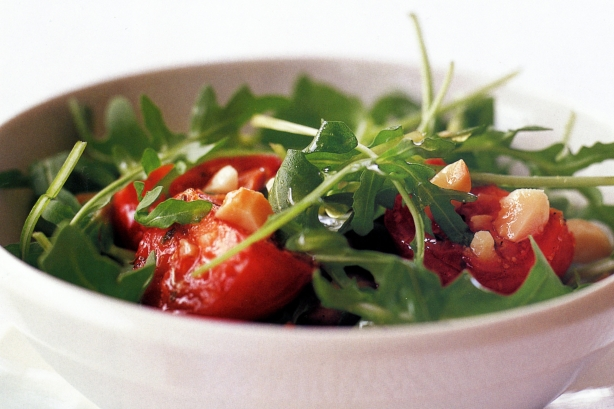
\includegraphics[scale=0.4]{./img/tomatorocketmacadamia.jpg}
%\end{figure}

\bigskip
\section*{Ingredients}

\begin{ingredients-list}
	\item 3 small vine-ripened tomatoes
		\begin{textblock*}{8cm}(8.5cm,-1.2cm) % {block width} (coords)
			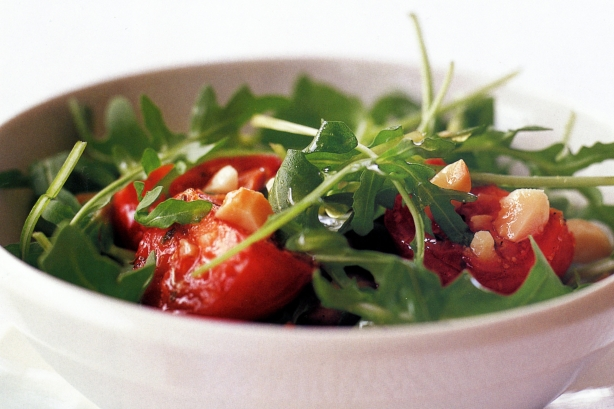
\includegraphics[scale=0.35]{./img/tomatorocketmacadamia.jpg}
		\end{textblock*}
	\item Sea Salt
	\item 300g wild rocket leaves
	\item 100g macadamia nuts, roasted, chopped
	\item 1 tsp. sugar
	\item 50ml olive oil
	\item 50ml macadamia nut oil*
	\item 40ml (2 tbsp.) white wine vinegar
	\item 1 tsp. Dijon mustard
	\item 2 tsp. Australian honey
\end{ingredients-list}

\section*{Directions}
\begin{enumerate}
	\item Cut tomatoes into quarters; add sugar, salt and pepper. Heat a non-stick pan on high heat and fry tomatoes cut-side down until slightly charred. Set aside to cool.
	\item Place the rocket, tomato and macadamias in a serving bowl.
	\item  Place remaining ingredients in a bowl and whisk to combine. Toss the dressing through the salad and serve.
\end{enumerate}
%%End recipe

%%Start recipe
\newrecipe{Fattoush\\(Middle Eastern bread salad)}{http://www.taste.com.au/recipes/6769/fattoush+middle+eastern+bread+salad}

%\begin{figure}[h!]
%	\centering
%	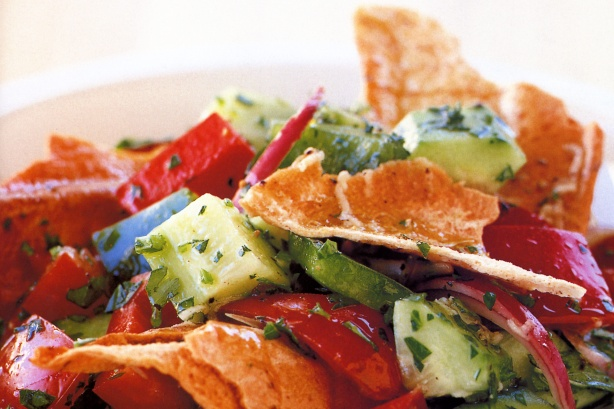
\includegraphics[scale=0.2]{./img/fattoush.jpg}
%\end{figure}
\bigskip
\section*{Ingredients}
\begin{ingredients-list}
	\item 3 small pita breads, halved
		\begin{textblock*}{8cm}(8.5cm,-1.2cm) % {block width} (coords)
			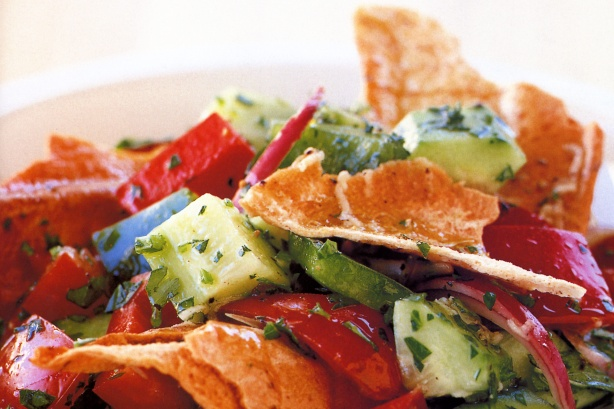
\includegraphics[scale=0.35]{./img/fattoush.jpg}
		\end{textblock*}
	\item 120ml (6 tbsp.) olive oil
	\item 2 garlic cloves, crushed
	\item 1 lemon, juiced
	\item 2 tbsp. chopped flat-leaf parsley
	\item 2 tbsp. chopped coriander leaves
	\item 2 tbsp. chopped, fresh mint leaves
	\item 1 red onion, sliced
	\item 5 tomatoes, seeded, cut into 1-2cm dice
	\item 1 telegraph cucumber, peeled, seeded,  diced into 1-2cm cubes
	\item 2 small green capsicums, seeded, diced into 1-2cm cubes
\end{ingredients-list}

\section*{Directions}
\begin{enumerate}
	\item Preheat oven to 190°C.
	\item Brush bread pieces with 2 tablespoons of the oil. Place on a baking tray and bake for 10-15 minutes until crisp and golden.
		Transfer to a plate lined with paper towel to drain and cool.
	\item Combine the garlic, lemon juice, remaining olive oil and herbs in a large bowl and season with salt and pepper.
		Add the onion, tomato, cucumber and capsicum and toss to combine.
		Just before serving, break the bread into rough pieces, add to the salad and toss well. Serve with grilled meat or fish.
\end{enumerate}
%%End Recipe

%%Start Recipe
\newrecipe{Tuna Pasta Salad}{}


\section*{Ingredients}
\begin{ingredients-list}
	\item 500g spiral pasta
	\item 1 tin (400g) of tuna
	\item 6 Sundried tomatoes cut into small strips
	\item 1 handful (20) kalamata Olives, sliced
	\item 2 Baby cos lettuce
	\item Grated parmesan cheese
	\item 50 g pine nuts
	\item 6 eggs.
	\item Anchovy Dressing from \hyperlink{salad_nicoise}{Salad nicoise recipe} on page \pageref{salad_nicoise}.
\end{ingredients-list}

\section*{Directions}
\begin{enumerate}
	\item Hard boil the eggs and leave to cool (in a sink of cold water)
	\item Toast the pine nuts in a dry frypan and set aside to cool.
	\item Cook pasta according to directions, and cool under running water.
	\item Drain the pasta well and place in large bowl with a little oil or some of the salad dressing.
		Toss lightly to prevent the pasta from sticking together.
	\item Add the chopped olives, sundried tomato strips and the remainder of the dressing and mix well.
	\item Peel the eggs and half or quarter them as desired
	\item Line bowls with the baby cos lettuce leaves and spoon in the pasta salad mixture.
	\item Garnish with eggs, pinenuts and parmesan cheese.
\end{enumerate}

%%End Recipe

%%End Chapter